\section{Consumer Evidence and Sensitivity Details}
\label{sec:consumer_evidence_details}
\subsection{Awesome-Selfhosted path corroboration}
The held-out frame comprises the remaining entries in the pinned Awesome-Selfhosted list after excluding all 40 pilot projects and repository keys that appear among earlier training endpoints. Each project is pinned to its public default HEAD when observed. We trace mandatory production dependencies from the root npm importer using committed lockfile formats 2 and 3. We corroborate the paths with npm Arborist's offline virtual tree. Workspaces, unsupported managers, unresolved paths and unavailable inputs contribute to the attrition ledger. The verification queue enumerates all distinct public package/version pairs corroborated by both implementations. We collect exact-version registry responses for this queue before matching any accounts to the portfolios. The registry fields describe observed maintainer-list associations during collection.

We recorded all 155 projects and pinned 154 commits. Thirty projects entered the paired parser comparison and 25 yielded at least one corroborated path. The implementations agreed on 6,388 package locations in the compared projects. Arborist returned a virtual tree for 18 additional projects declined by the custom parser. Across the agreed paths, exact-version registry observations produced a usable maintainer list for 3,287 of 3,299 requested versions.


\begin{figure}[t]
\centering
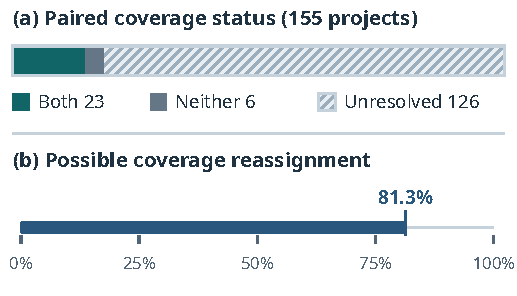
\includegraphics[width=\columnwidth]{consumer_holdout_evidence.pdf}
\caption{Paired consumer coverage evidence. The hatched segment shows unresolved pairs in the 155-application frame. The interval represents coverage reassignment compatible with the available evidence. All five-account tie choices give the same counts and bounds.}
\label{fig:consumer_holdout_evidence}
\end{figure}
\par Figure~\ref{fig:consumer_holdout_evidence} records the original evidence categories in this frame.

\subsection{YunoHost comparison with broader lockfile support}
The second frame comprises 215 upstream YunoHost projects with pinned root package manifests. We excluded earlier repository keys and duplicate pinned commits. Lockfile intake yielded 108 npm and 44 pnpm candidates. All 215 projects contribute to the paired comparison.

For npm, we compare effective ranges from Arborist's virtual tree with checks against the committed dependency declarations, lockfile locations and pinned workspace manifests. The root walk follows verified links to local workspaces when those links are on a mandatory production path. Separate workspace importers are diagnostic because the catalog does not establish which importer is deployed. For pnpm lockfile format 9, we compare paths of up to three mandatory edges against the native offline listing. The depth limit lets those paths establish positive witnesses. A negative requires complete npm evidence within the supported root scope and an observed registry join for every retained witness.

We froze the comparison and the verification scope before acquiring the workspace manifests and observing the exact-version registry metadata used for scoring. A path's registry identity requires a canonical public npm tarball URL or an exact match between the lockfile's SHA-512 identifier and the registry response. We join maintainer associations after collection. Both frames measure committed dependency declarations and registry associations at the time of observation. The different intake and extraction rules limit direct comparisons between frames.

On the same 108 npm candidates, the earlier reader returned corroborated locations for 50 projects and the expanded reader for 67. The readings share 8,158 package locations. The expanded procedure adds 5,463 locations in 19 projects, including three with root workspaces. It also leaves 316 previously corroborated locations unresolved in two projects. This comparison measures where the two procedures produce evidence on the same inputs.

The workspace collection returned all 15 requested manifests. The registry collection returned usable maintainer lists for 9,968 of 9,987 exact versions. Ninety projects have at least one registry-linked path. Seventy-two have complete path and registry evidence under the supported root scope. Positive witnesses under both portfolios also resolve pairs in projects with incomplete trees.

% Values from yunohost-v2, yunohost-yarn-classic and yunohost-empty-pnpm-roots results.json.
\begin{table}[t]
\centering
\footnotesize
\caption{Paired coverage in the 215-project YunoHost frame. Each column compares the name portfolio against a different additive-optimal version portfolio. Bounds account for unresolved pairs.}
\label{tab:yunohost_consumer_holdout}
\setlength{\tabcolsep}{3pt}
\begin{tabularx}{\linewidth}{@{}Yrrr@{}}
\toprule
Measure & Primary & Alt.~1 & Alt.~2\\
\midrule
\multicolumn{4}{@{}l}{\textit{Initial npm and pnpm analysis}}\\
Documented under both & 70 & 67 & 71\\
Documented name only & 4 & 7 & 3\\
Documented version only & 2 & 1 & 2\\
Documented under neither & 139 & 140 & 139\\
\addlinespace
Fully resolved pairs & 112 & 110 & 112\\
Fully resolved differences & 5 & 5 & 4\\
Turnover bounds (\%) & $[2.3,50.2]$ & $[2.3,51.2]$ & $[1.9,49.8]$\\
Net change bounds (pp) & $[-48.4,47.0]$ & $[-50.2,46.0]$ & $[-47.9,47.4]$\\
\addlinespace
\multicolumn{4}{@{}l}{\textit{After adding Yarn Classic evidence}}\\
Follow-up resolved pairs & 129 & 127 & 129\\
Follow-up turnover (\%) & $[2.3,42.3]$ & $[2.3,43.3]$ & $[1.9,41.9]$\\
Follow-up net change (pp) & $[-40.0,38.6]$ & $[-41.9,37.7]$ & $[-39.5,39.1]$\\
\addlinespace
\multicolumn{4}{@{}l}{\textit{Empty pnpm root sensitivity}}\\
Sensitivity resolved pairs & 145 & 143 & 145\\
Sensitivity turnover (\%) & $[2.3,34.9]$ & $[2.3,35.8]$ & $[1.9,34.4]$\\
Sensitivity net change (pp) & $[-32.6,31.2]$ & $[-34.4,30.2]$ & $[-32.1,31.6]$\\
\bottomrule
\end{tabularx}
\end{table}


In the primary comparison, 70 applications have documented hits under both portfolios and six have hits under just one. Five of those six are confirmed differences from fully checked roots (three name-only and two version-only). At least four pairs differ under each alternative cutoff tie, and three projects differ under all three choices. A post hoc check found a positive witness location corroborated by the earlier npm reader for every confirmed difference. The identical-portfolio control has zero turnover. The 103 unresolved primary pairs leave the total net coverage change compatible with either direction (Table~\ref{tab:yunohost_consumer_holdout}).

\subsection{Yarn Classic follow-up}
After the initial YunoHost analysis, we froze a follow-up protocol for its 35 Yarn candidates before collecting new registry evidence. Two lockfile readers checked the declared SemVer paths from each root. We excluded newer Yarn formats, workspace importers and edges affected by selective resolutions. Paths require canonical registry identifiers, SHA-512 agreement for Yarn mirror artifacts, and corroboration of transitive declarations against exact-version registry records. Yarn contributes positive witnesses only.

The readers agreed on 20 eligible lockfiles. Of 3,557 exact-version requests, 3,555 yielded usable maintainer lists. Nineteen applications have a registry-linked path. The added evidence resolves 17 further common hits in the primary comparison, raising the resolved count from 112 to 129. Two more applications have one documented portfolio hit and an unresolved counterpart. The turnover interval narrows to 2.3--42.3\% and the net interval to $-40.0$ to $+38.6$ percentage points. Both alternative cutoff choices show the same 17-pair increase (Table~\ref{tab:yunohost_consumer_holdout}). The follow-up retains the original observations for all other projects. Its bounds quantify the change from adding Yarn evidence collected separately.

\subsection{Sensitivity to empty pnpm roots}
The primary protocol uses pnpm paths to establish positive witnesses.
Among the 86 unresolved primary pairs after the Yarn follow-up, 23 had pnpm lockfile evidence. Sixteen of these had zero witnesses in a successful root comparison.
In a post hoc sensitivity analysis, we checked each of those 16 pinned
manifests and pnpm v9 root importers for regular dependency declarations.
All 16 had empty mandatory roots in both files. Thirteen declared
development dependencies. The other three had no development
declarations in the manifest. Under the mandatory root scope, these 16
applications are common negatives.

Adding these common negatives resolves 145 of 215 primary pairs and
leaves 70 unresolved. The turnover interval is 2.3--34.9\% and the net
interval is $-32.6$ to $+31.2$ percentage points. The five confirmed
differences persist. Table~\ref{tab:yunohost_consumer_holdout} also
reports the two alternative cutoff choices. The sensitivity covers
regular dependencies declared at the pinned root importer. Development
dependencies, other importers and release contents are outside this check.

\subsection{Newer Yarn, missing lockfiles and Bun}
We ran two further post hoc checks on unresolved projects. For all 14
newer Yarn candidates, we compared root declarations with the
\texttt{workspace:.} entry. Six roots had zero regular, optional,
peer or bundled dependencies. Their lock entries contain exactly the
development declarations from the pinned manifests. For all 18
projects without an available root lockfile, we checked the manifests
and lockfile receipts. Nine had empty production manifests, no declared
workspaces, and HTTP 404 receipts for all tested root lockfile names and
the pnpm workspace file. An empty declaration establishes a zero for
the root-scope estimand even when the capture has no lockfile. Taken
together, these checks add 15 common negatives and increase the number
of resolved primary pairs to 160 (Table~\ref{tab:yunohost_consumer_holdout}).

We also screened all six unresolved Bun projects for direct evidence.
Two had supported text lockfiles and matching root declarations
without overrides or patches. Across these two projects, 14 exact
versions matched the SHA-512 values in retained npm registry receipts.
The locked \texttt{p-queue} 10.0.0 at project Y473 supplies a
shared hit for the name selection and all three version alternatives.
This positive-only check resolves one more project. The combined
sensitivity resolves 161 of 215 primary pairs. Feasible turnover is
2.3--27.4\%, and net change is $-25.1$ to $+23.7$ percentage points.
The five confirmed coverage changes persist. The results concern
declared paths from a pinned root. Other workspace roots and
dependencies introduced during packaging are outside this comparison.

\subsection{Checks on unresolved npm roots}
We examined all 17 unresolved npm projects for empty production
roots or additional verifiable identities. Three root manifests had no
regular, optional, peer or bundled dependencies and corroborating
lockfile evidence. Two had matching root declarations in v3 lockfiles.
The third had a v1 lockfile with all 806 entries marked
development-only and locked root development versions satisfying the
manifest ranges. We left two other empty manifests unresolved because
their version labels disagree with the lockfiles.

Two projects had complete path extraction but incomplete registry
identity. We found 62 locations across them with neither a tarball URL
nor usable SHA-512. Checking direct v1 dependencies against retained
registry receipts supplied no additional hits. Adding the three
corroborated zeros resolves 164 primary pairs and leaves 51 unresolved.
The turnover bounds narrow to 2.3--26.0\%, and net change remains
compatible with either direction ($-23.7$ to $+22.3$ percentage points).
This is a post hoc sensitivity within the same declared root scope.

